\documentclass[answers]{exam}

%% Language and font encodings
\usepackage[english]{babel}
\usepackage[utf8x]{inputenc}
\usepackage[T1]{fontenc}
\usepackage[nomarkers,figuresonly]{endfloat}

%% Sets page size and margins
\usepackage[a4paper,margin=2cm]{geometry}

%% Useful packages
\usepackage{amsmath}
\usepackage{graphicx}
\usepackage{paralist}
\setlength\FrameSep{4pt}

\newcommand{\ptm}[1]{p_{\textsc{TM}}(#1)}
\newcommand{\plm}[1]{p_{\textsc{LM}}(#1)}
\DeclareMathOperator*{\argmax}{arg\,max}

\begin{document}
\begin{questions}
\question[10]{Experiment with stack pruning parameters. What is their affect on...}
\begin{framed}
\begin{compactenum}[a.]
\item log-probabilities:\\
  The log-probabilities go up with increases in $s$ and $k$, though there seems
  to be no significant increase past either $s > 10$ or $k > 10$. The
  log-probabilities plateau at around this point. 
\item speed:\\
  The time seems to go up \emph{at most} linearly with increases in $s$, though
  the curve gets steeper with increases in $k$. Note: in the graphs, both the
  time and the stack size are plotted logarithmically.
\item translations:
\item maximum log-probability:\\
  The log-probability plateaus at $-1353.247828$.
\end{compactenum}
(See figure \ref{fig:exp-baseline}.)
\end{framed}


\question[15]{Define a new dynamic program for Part 2.}
\begin{framed}
  \begingroup\raggedright
  First, let us define some notation for the sum of the log-probabilities of the
  sequence $e_{1}\dots e_{k}e$ following $e'$ according to the language model: 
  \par\endgroup
  \(\!
  \begin{aligned}
    \log{\plm{e_{1}\dots e_{k}e \mid e'}}
    = \log{\plm{e_{1} \mid e'}}
    + \sum_{i=1}^{k-1}{\log{\plm{e_{i+1} \mid e_{i}}}}
    + \log{\plm{e \mid e_{k}}}
  \end{aligned}
  \)
  \\
  \begingroup\raggedright
  Secondly, we let $h(i,e) = s(0,0,i,e)$, and we define $s(k,j,i,e)$, for $k =
  j = 0 \lor k < j$, as follows:
  \par\endgroup
  \(\!
  \begin{aligned}
    &s(0,0,0,e) =
    \begin{cases}
      \epsilon         &\text{if }e = \text{START}\\
      \text{undefined} &\text{otherwise}
    \end{cases}
  \end{aligned}
  \)
  \(\!
  \begin{aligned}
    &s(0,0,i,e) = \argmax_{s(k,j,i',e')e_{1}\dots e_{n}e}
    &&\log{p(s(k,j,i',e'))} + \log{\plm{e_{1}\dots e_{n}e \mid e'}}
    \\& &&+
    \begin{cases}
      \log{\ptm{f_{i'+1}\dots f_{i} \mid e_{1}\dots e_{n}e}}
      &\text{if }k = 0 \land j = 0
      \\
      \log{\ptm{f_{k}\dots f_{j-1} \mid e_{1}\dots e_{n}e}}
      &\text{if }i' = i
    \end{cases}
    \\
    &s(k,j,i,e) =
    \argmax_{s(0,0,i',e')e_{1}\dots e_{n}e}
    &&\log{p(s(0,0,i',e'))} + \log{\plm{e_{1}\dots e_{n}e \mid e'}} 
    \\& &&+\;\log{\ptm{f_{j}\dots f_{i} \mid e_{1}\dots e_{n}e}}
  \end{aligned}
  \)
  \\
  \begingroup\raggedright
  Note that $s(0,0,i,e)$ does \emph{not} denote a translation state with a hole
  in the $k^{th}$ position, as the second argument is the index of the first
  word \emph{after} the gap. It denotes a translation state without a gap.
  \par\endgroup
\end{framed}


\question[5]{What is the complexity of your Part 2 decoder? Explain your reasoning.}
\begin{framed}
\end{framed}


\question[5]{What is the mapping from hypothesis objects to stacks for Part 2?}
\begin{framed}
  Hypothesis objects are mapped to stacks as $s(k,j,i,e)\mapsto i - (k - j)$, as
  we need to subtract the number of words in the gap ($k - j$) from the number
  of words covered ($i$). Since $h(i,e) = s(0,0,i,e)$, $h(i,e)\mapsto i$ as in
  the previous model.
\end{framed}


\addtocounter{question}{1}
\question[15] Experiment with stack pruning parameters for Part 2. What is their affect on...
\begin{framed}
\begin{compactenum}[a.]
\item log-probabilities:\\
  The log-probabilities go up with increases in $s$ and $k$, though there seems
  to be no significant increase past $s > 50$ and $k > 10$. The
  log-probabilities plateau at this point. 
\item speed:
  The time seems to go up \emph{at most} linearly with increases in $s$, though
  the curve gets steeper with increases in $k$.
\item translations:
\item maximum log-probability:\\
  The log-probability plateaus at $-1300.526262$.
\end{compactenum}
(See figure \ref{fig:exp-part2}.)
\end{framed}


\question[10]{Define a new dynamic program for Part 3.}
\begin{framed}
  For Part 2, our program had the choice of either translating the next phrase,
  or leaving a hole---of exactly one phrase---and translating a phrase following
  that. However, if it chooses to leave a hole, it had to translate the hole
  immediately after, as a consequence of the swapping constraint. 
  The description of Part 3 implies that \emph{this} program can translate any
  number of phrases before going back and translating the hole, as long as it
  never left more than one hole, and never one of more than one phrase. 
  \\
  The definition of Part 3 is very similar to that of Part 2, sharing---for
  starters---the same auxiliary definition and the same basic form of
  $s(k,j,i,e)$, which I will not repeat here. The only real difference is in the
  final equation, in which it is now possible to continue translating phrases
  while there is a hole.
  \\
  \\
  \(\!
  \begin{aligned}
    &s(0,0,0,e) = \ldots\\
    &s(0,0,i,e) = \ldots\\
    &s(k,j,i,e) =
    \argmax_{s(k',j',i',e')e_{1}\dots e_{n}e}
    &&\log{p(s(k',j',i',e'))} + \log{\plm{e_{1}\dots e_{n}e \mid e'}} 
    \\& &&+
    \begin{cases}
      \log{\ptm{f_{j}\dots f_{i} \mid e_{1}\dots e_{n}e}}
      &\text{if }k' = 0 \land j' = 0
      \\
      \log{\ptm{f_{k}\dots f_{j-1} \mid e_{1}\dots e_{n}e}}
      &\text{if }i' = i
    \end{cases}
  \end{aligned}
  \)
\end{framed}


\question[5]{What is the computational complexity of your Part 3 decoder?}
\begin{framed}
\end{framed}


\question[5]{What is the mapping from hypothesis objects to stacks for Part 3?}
\begin{framed}
  Hypothesis objects are mapped to stacks in the same way as in Part 2.
\end{framed}


\addtocounter{question}{1}
\question[5]{What is the maximum log-probability your Part 3 decoder can obtain? What do you conclude?}
\begin{framed}
  $-1278.680068$, with $s = 2000, k = 100$. For further increases of $s$,
  the score does not improve, and given the fact that the score does not change
  between $s = 1000, k = 50$ and $s = 1000, k = 100$ I am guessing that further
  increases of $k$ will not make a difference either.
  Therefore, this is likely the best log-probability which my Part 3 decoder can
  obtain, and is significantly better than the top scores for my Part 2 decoder.
  However, with a runtime of just under half an hour, $s$ is impractically large
  at this point. Especially since we can get a score of $-1281.046784$ at
  \emph{one-tenth} the runtime using $s = 500, k = 10$. 
  \\
  All in all, our scores tell us that the Part 3 decoder is an improvement over
  the Part 2 decoder: the difference between the best for Part 3 and Part 2 is
  about half as big as the difference between Part 2 and Part 1.
  \\
  If we think about it from a linguistic perspective, this makes sense. Our
  swapping decoder would fix a lot of things such as French adjectives, which
  are binary swaps. Longer distance dependences, which I suppose are less
  frequent, would still be translated to the wrong position. The thing which may
  not make sense is that we can only move single phrases. For instance, if we
  translate from an SVO language to an SOV language, we may want to move a
  complex object. We would be able to do this \emph{only} if the object, in its
  entirety, were present in the phrase table. A program allowing a sequence of
  phrases to be displaced might work better, but also would massively inflate
  the number of possible translations. A program which uses swaps in the parse
  tree would perform better, but we cannot just assume we have a parse tree.
  \\
  \\
  (See figure \ref{fig:exp-part3}. Data for $s > 1000$ not included.)
\end{framed}
\end{questions}


% figures

\begin{figure}
  \centering
  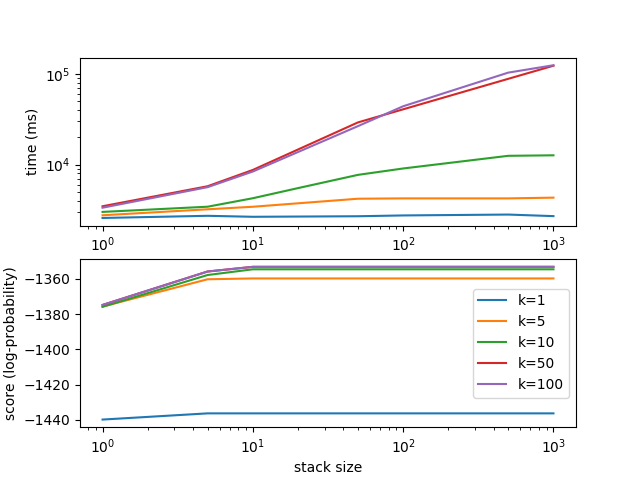
\includegraphics{fig-default}
  \caption[Experiment (baseline).]{Experiment with stack pruning parameters
    (baseline).}
  \label{fig:exp-baseline}
\end{figure}

\begin{figure}
  \centering
  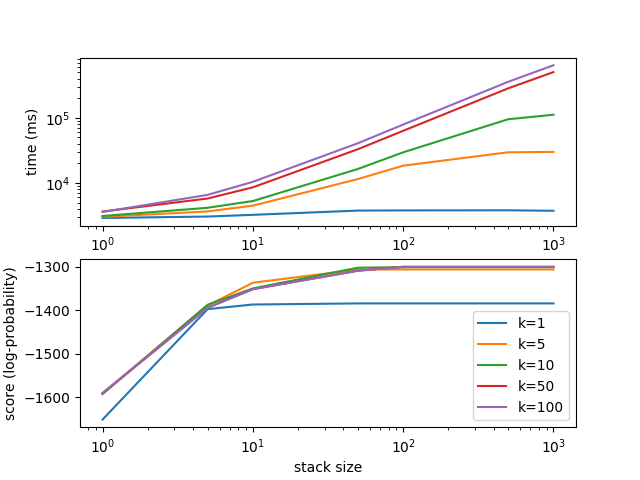
\includegraphics{fig-part2}
  \caption[Experiment (baseline).]{Experiment with stack pruning parameters
    (part2).}
  \label{fig:exp-part2}
\end{figure}

\begin{figure}
  \centering
  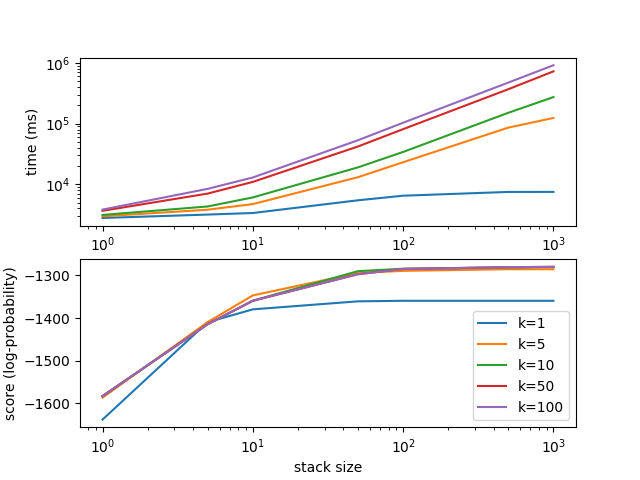
\includegraphics{fig-part3}
  \caption[Experiment (baseline).]{Experiment with stack pruning parameters
    (part3).}
  \label{fig:exp-part3}
\end{figure}


\end{document}